\documentclass[class=report,crop=false]{standalone}
\usepackage[screen]{prkbook}
\usepackage[]{epsdice}

\begin{document}
\renewcommand{\chtag}{Question}
\renewcommand{\myclass}{pk}
\newcommand{\myyear}{2018}
\setlength{\columnseprule}{0pt}
%====================================================================
\chapitre[Olympiade Mathématiques Belge {\myyear} - Mini]{Olympiade Mathématique Belge {\myyear} - Mini - Eli}
%====================================================================
%%%%%%%%%%%%%%%%%%%%%%%%%%%%%%%%%%%%%%%%%%%%%%%%%%%%%%%%%%%%%%%%
\subsection*{Extrait du règlement du concours}
\ombintro
\subsection*{Le questionnaire éliminatoire \myyear}
%---------------------------------------------------------------

\begin{Exercise}[title={},label={\pktag\the\value{Exercise}}]
$1-\left(\frac{1}{2}\right)^2=$
\begin{multicols}{5}
\begin{enumerate}[label=\Alph* : ]
  \item $0$
  \item $\frac{1}{4}$
  \item $\frac{1}{2}$
  \item $\frac{3}{4}$
  \item $\frac{5}{4}$
\end{enumerate}
\end{multicols}
\end{Exercise}
\begin{Answer}[ref=\ExerciseLabel]
A : $\frac{3}{4}$\\\ws\\
$1-\left(\frac{1}{2}\right)^2=1-\frac{1}{4}=\frac{3}{4}$
\end{Answer}

\begin{Exercise}[title={},label={\pktag\the\value{Exercise}}]
Combien peut-il y avoir au maximum de lundis dans une période de 75 jours consécutifs?
\begin{multicols}{5}
\begin{enumerate}[label=\Alph* : ]
  \item $10 $
  \item $11 $
  \item $12 $
  \item $13 $
  \item $15 $
\end{enumerate}
\end{multicols}
\end{Exercise}
\begin{Answer}[ref=\ExerciseLabel]
B : $11$\\\ws\\
$75=7\cdot10+5$ ; 75 jours consécutifs forment 10 semaines et 5 cinq jours ; $10+1=11$ lundis au maximum.
\end{Answer}

\begin{Exercise}[title={\srp},label={\pktag\the\value{Exercise}}]
Un car peut transporter 62 personnes (en plus du chauffeur). Si une école de 692 élèves et 35 de leurs professeurs doivent partir en excursion, combien faudra-t-il de cars de ce type, au minimum, pour que tous aient une place assise?
\end{Exercise}
\begin{Answer}[ref=\ExerciseLabel]
$12$\\\ws\\
$(692+35):62=727:62=(682+45):62=11+\frac{45}{62}$ ; il faudra donc $12$ cars.
\end{Answer}

\begin{Exercise}[title={},label={\pktag\the\value{Exercise}}]
Une salle de cinéma compte onze rangées de sièges, numérotées de 1 à 11. Les rangées dont le numéro est impair ont 15 sièges chacune, tandis que les rangées dont le numéro est pair ont 16 sièges chacune. Combien y a-t-il de sièges dans le cinéma?
\begin{multicols}{5}
\begin{enumerate}[label=\Alph* : ]
  \item $76 $
  \item $165 $
  \item $170 $
  \item $171 $
  \item $186 $
\end{enumerate}
\end{multicols}
\end{Exercise}
\begin{Answer}[ref=\ExerciseLabel]
C : $170$\\\ws\\
$6\cdot15+5\cdot16=90+80=170$ ; il y a 170 sièges dans le cinéma.
\end{Answer}

\begin{Exercise}[title={},label={\pktag\the\value{Exercise}}]
\begin{minipage}{0.7\linewidth}
Une grille $3\times 3$ est remplie par des nombres un, deux et trois écrits de trois manières: en chiffres indo-arabes,
en chiffres romains et en faces de dés. Dans chaque ligne et dans chaque colonne se trouvent les trois valeurs et les trois écritures. Que contient la case centrale (grisée)?
\end{minipage}
\begin{minipage}{0.3\linewidth}
\begin{center}
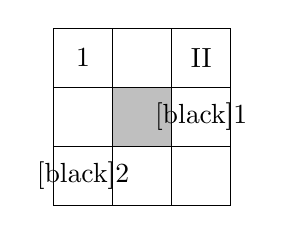
\begin{tikzpicture}[scale=0.75]
\draw[] (0,0) rectangle (1,1) node[pos=.5] {\epsdice[black]{2}};
\draw[] (1,0) rectangle (2,1) node[pos=.5] {};
\draw[] (2,0) rectangle (3,1) node[pos=.5] {};

\draw[] (0,1) rectangle (1,2) node[pos=.5] {};
\draw[fill=black!25] (1,1) rectangle (2,2) node[pos=.5] {};
\draw[] (2,1) rectangle (3,2) node[pos=.5] {\epsdice[black]{1}};

\draw[] (0,2) rectangle (1,3) node[pos=.5] {1};
\draw[] (1,2) rectangle (2,3) node[pos=.5] {};
\draw[] (2,2) rectangle (3,3) node[pos=.5] {II};
\end{tikzpicture}
\end{center}
\end{minipage}\\

\begin{multicols}{5}
\begin{enumerate}[label=\Alph* : ]
  \item $2 $
  \item $3 $
  \item \epsdice[black]{3}
  \item I 
  \item III 
\end{enumerate}
\end{multicols}
\end{Exercise}
\begin{Answer}[ref=\ExerciseLabel]
A : 2\\\ws
\begin{center}
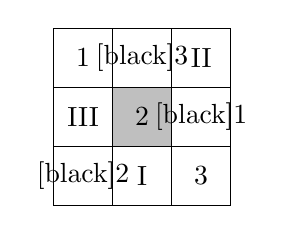
\begin{tikzpicture}[scale=0.75]
\draw[] (0,0) rectangle (1,1) node[pos=.5] {\epsdice[black]{2}};
\draw[] (1,0) rectangle (2,1) node[pos=.5] {I};
\draw[] (2,0) rectangle (3,1) node[pos=.5] {3};

\draw[] (0,1) rectangle (1,2) node[pos=.5] {III};
\draw[fill=black!25] (1,1) rectangle (2,2) node[pos=.5] {2};
\draw[] (2,1) rectangle (3,2) node[pos=.5] {\epsdice[black]{1}};

\draw[] (0,2) rectangle (1,3) node[pos=.5] {1};
\draw[] (1,2) rectangle (2,3) node[pos=.5] {\epsdice[black]{3}};
\draw[] (2,2) rectangle (3,3) node[pos=.5] {II};
\end{tikzpicture}
\end{center}
\end{Answer}

\begin{Exercise}[title={\srp},label={\pktag\the\value{Exercise}}]
La somme des chiffres de $2018$ est divisible par $11$. Combien d'années faudra-t-il attendre pour que cela se reproduise pour la première fois?
\end{Exercise}
\begin{Answer}[ref=\ExerciseLabel]
9 \\\ws\\
Il faudra attendre 9 ans $(2018+9=2027)$ car la somme des chiffres de 2027 est égale à $2+0+2+7=11$.
\end{Answer}

\begin{Exercise}[title={\srp},label={\pktag\the\value{Exercise}}]
Fred ouvre sa tirelire. Il y découvre $11.20\eur$ en pièces de monnaie. Il y a le même nombre de pièces de 1 centime, de 5 centimes et de 10 centimes; il n'y a pas de pièce d'une autre valeur. Combien y a-t-il de pièces de monnaie de chaque sorte?
\end{Exercise}
\begin{Answer}[ref=\ExerciseLabel]
70 \\\ws\\
$0.01\cdot x+0.05\cdot x+0.10\cdot x = 11.20\iff 0.16\cdot x=11.20\iff x=1120:16\iff x=70$ pièces de monnaie.
\end{Answer}

\begin{Exercise}[title={\srp},label={\pktag\the\value{Exercise}}]
La longueur des arêtes d'un cube est multipliée par $5$. Par combien est multiplié son volume?
\end{Exercise}
\begin{Answer}[ref=\ExerciseLabel]
125 \\\ws\\
$V_\text{avant}=a^3$ ; $V_\text{après}=(5\cdot a)^3=125\cdot a^3 = 125\cdot V_\text{avant}$ ; le volume est multiplié par $125$.
\end{Answer}

\begin{Exercise}[title={},label={\pktag\the\value{Exercise}}]
Pierre et Paul fêtent ensemble leurs anniversaires au restaurant avec quelques amis. S'ils divisent l'addition entre tous, la part de chacun est de $30\eur$. Mais à la fin du diner, les amis insistent pour que Pierre et Paul ne paient pas; chacun des autres paie alors $40\eur$. Combien de personnes étaient présentes à ce repas, en plus de Pierre et de Paul?
\begin{multicols}{5}
\begin{enumerate}[label=\Alph* : ]
  \item $6 $
  \item $8 $
  \item $10 $
  \item $30 $
  \item $40 $
\end{enumerate}
\end{multicols}
\end{Exercise}
\begin{Answer}[ref=\ExerciseLabel]
A : $6$ \\\ws\\
$30\cdot(x+2) = 40\cdot x\iff 30x+60=40x\iff 10x=60\iff x=6$ ; 6 personnes étaient présentes à ce repas, en plus de Pierre et de Paul.
\end{Answer}

\begin{Exercise}[title={},label={\pktag\the\value{Exercise}}]
Quel est le double de $2.3\cdot10^4$?
\begin{multicols}{5}
\begin{enumerate}[label=\Alph* : ]
  \item $4.6\cdot10^4 $
  \item $2.3\cdot10^8 $
  \item $4.6\cdot10^8 $
  \item $2.3\cdot20^4 $
  \item $4.6\cdot20^4 $
\end{enumerate}
\end{multicols}
\end{Exercise}
\begin{Answer}[ref=\ExerciseLabel]
A : $4.6\cdot10^4$\\\ws\\
$2.3\cdot10^4\cdot2 = 2.3\cdot2\cdot10^4=4.6\cdot10^4$
\end{Answer}

\begin{Exercise}[title={},label={\pktag\the\value{Exercise}}]
Dans le tableau ci-dessous, un nombre dans une case blanche est la somme des nombres situés dans les deux cases blanches les plus proches de la rangée précédente (au-dessus); par exemple, le 9 est la somme de 4 et de 5. Que vaut $x$?
\begin{center}
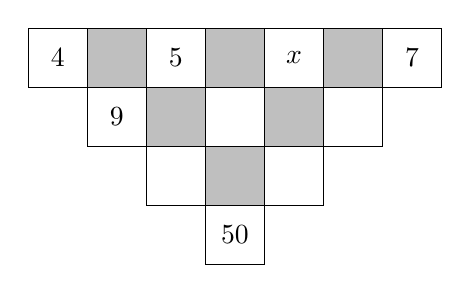
\begin{tikzpicture}[scale=0.75]
\draw[] (0,0) rectangle (1,1) node[pos=.5] {4};
\draw[fill=black!25] (1,0) rectangle (2,1);
\draw[] (2,0) rectangle (3,1) node[pos=.5] {5};
\draw[fill=black!25] (3,0) rectangle (4,1);
\draw[] (4,0) rectangle (5,1) node[pos=.5] {$x$};
\draw[fill=black!25] (5,0) rectangle (6,1);
\draw[] (6,0) rectangle (7,1) node[pos=.5] {7};

\draw[] (1,0) rectangle (2,-1) node[pos=.5] {9};
\draw[fill=black!25] (2,0) rectangle (3,-1);
\draw[] (3,0) rectangle (4,-1);
\draw[fill=black!25] (4,0) rectangle (5,-1);
\draw[] (5,0) rectangle (6,-1);

\draw[] (2,-1) rectangle (3,-2);
\draw[fill=black!25] (3,-1) rectangle (4,-2);
\draw[] (4,-1) rectangle (5,-2);

\draw[] (3,-2) rectangle (4,-3) node[pos=.5] {50};
\end{tikzpicture}
\end{center}

\begin{multicols}{5}
\begin{enumerate}[label=\Alph* : ]
  \item $4 $
  \item $6 $
  \item $7 $
  \item $8 $
  \item $10 $
\end{enumerate}
\end{multicols}
\end{Exercise}
\begin{Answer}[ref=\ExerciseLabel]
D : 8\\\ws
\begin{center}
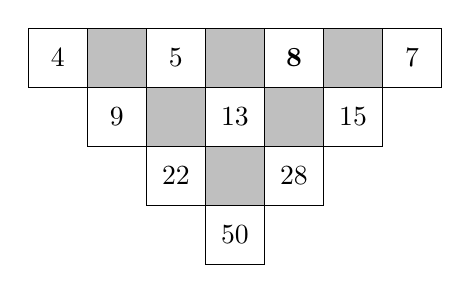
\begin{tikzpicture}[scale=0.75]
\draw[] (0,0) rectangle (1,1) node[pos=.5] {4};
\draw[fill=black!25] (1,0) rectangle (2,1);
\draw[] (2,0) rectangle (3,1) node[pos=.5] {5};
\draw[fill=black!25] (3,0) rectangle (4,1);
\draw[] (4,0) rectangle (5,1) node[pos=.5] {\textbf{8}};
\draw[fill=black!25] (5,0) rectangle (6,1);
\draw[] (6,0) rectangle (7,1) node[pos=.5] {7};

\draw[] (1,0) rectangle (2,-1) node[pos=.5] {9};
\draw[fill=black!25] (2,0) rectangle (3,-1);
\draw[] (3,0) rectangle (4,-1) node[pos=.5] {13};
\draw[fill=black!25] (4,0) rectangle (5,-1);
\draw[] (5,0) rectangle (6,-1) node[pos=.5] {15};

\draw[] (2,-1) rectangle (3,-2) node[pos=.5] {22};
\draw[fill=black!25] (3,-1) rectangle (4,-2);
\draw[] (4,-1) rectangle (5,-2) node[pos=.5] {28};

\draw[] (3,-2) rectangle (4,-3) node[pos=.5] {50};
\end{tikzpicture}
\end{center}
\end{Answer}

\begin{Exercise}[title={},label={\pktag\the\value{Exercise}}]
L'aire du parallélogramme ci-dessous est 6. Que vaut l'aire ombrée?
\begin{center}

\begin{tikzpicture}[scale=1]
    
    \tkzDefPoint(0,0){O}
    \tkzDefPoint(0.5,2){D1}
    \tkzDefPoint(1.5,2){A}
    \tkzDefPoint(3.5,2){B}
    \tkzDefPoint(4,2){D2}
    
    \tkzDefPoint(3.5,0){D3}
    \tkzDefPoint(2.5,0){D4}
    
    \tkzLabelPoint[above](A){$A$}
    \tkzLabelPoint[above](B){$B$}
    \tkzDrawPolygon(O,D1,A,B,D2,D3)
    \tkzDrawPolygon[fill=black!25](A,D4,O)
    \tkzDrawPolygon[fill=black!25](B,D3,D4)

\end{tikzpicture}  
\end{center} 

\begin{multicols}{3}
\begin{enumerate}[label=\Alph* : ]
  \item $1 $
  \item $2 $
  \item $3 $
  \item $4 $
  \item Elle dépend des positions
  \item[] de $A$ et $B$.
\end{enumerate}
\end{multicols}
\end{Exercise}
\begin{Answer}[ref=\ExerciseLabel]
C : 3\\\ws
\begin{center}

\begin{tikzpicture}[scale=1]
    \tkzDefPoint(0,0){O}
    \tkzDefPoint(0.5,2){D1}
    \tkzDefPoint(1.5,2){A}
    \tkzDefPoint(3.5,2){B}
    \tkzDefPoint(4,2){D2}
    \tkzDefPoint(1.5,0){H}
    
    \tkzDefPoint(3.5,0){D3}
    \tkzDefPoint(2.5,0){D4}
    
    \tkzDrawPolygon(O,D1,A,B,D2,D3)
    \tkzDrawPolygon[fill=black!25](A,D4,O)
    \tkzDrawPolygon[fill=black!25](B,D3,D4)
    
    \tkzLabelPoint[above](A){$A$}
    \tkzLabelPoint[above](B){$B$}
    \tkzLabelSegment[below](D4,O){$b_1$}
    \tkzLabelSegment[below](D3,D4){$b_2$}
    \tkzLabelSegment[right](A,H){$h$}
    \tkzDrawSegment[dashed](A,H)
\end{tikzpicture}  
\end{center} 
$A=A_1+A_2=\frac{1}{2}\cdot b_1\cdot h+\frac{1}{2}\cdot b_2\cdot h=\frac{1}{2}\cdot h\cdot\left(b_1+b_2\right)=\frac{1}{2}\cdot h\cdot b=\frac{1}{2}\cdot A_\text{parallélogramme}=\frac{1}{2}\cdot 6=3$
\end{Answer}

\begin{Exercise}[title={},label={\pktag\the\value{Exercise}}]
Sur une ligne de chemin de fer, la distance entre les villes $A$ et $B$ est de $70\,km$. Une ville $C$ est située sur la ligne, entre $A$ et $B$, à $40\,km$ de $A$. Si un train, roulant à vitesse constante, est parti de $A$ à 10h07 et arrivé en $B$ à 10h49, à quelle heure est-il passé en $C$?
\begin{multicols}{5}
\begin{enumerate}[label=\Alph* : ]
  \item 10h21
  \item 10h24
  \item 10h27
  \item 10h31
  \item 10h35
\end{enumerate}
\end{multicols}
\end{Exercise}
\begin{Answer}[ref=\ExerciseLabel]
D : 10h31\\\ws\\
$\frac{42}{70}=\frac{x}{40}\iff x=\frac{42\cdot40}{70}\iff x=6\cdot 4\iff x=24$ ; le train passe à \og{}10h07 + 00h24 = 10h31\fg{} en $C$. 
\end{Answer}

\begin{Exercise}[title={},label={\pktag\the\value{Exercise}}]
Si $m$ et $n$ désignent des nombres naturels impairs, alors, parmi les nombres suivants, lequel est forcément impair?
\begin{multicols}{3}
\begin{enumerate}[label=\Alph* : ]
  \item $m+n $
  \item $m-n $
  \item $m\cdot n $
  \item $3m+7n $
  \item Aucun des précédents.
  \item[] 
\end{enumerate}
\end{multicols}
\end{Exercise}
\begin{Answer}[ref=\ExerciseLabel]
C : $m\cdot n$\\\ws\\
$m\cdot n=\left(2p+1\right)\cdot\left(2q+1\right)=4pq+2p+2q+1=\underbrace{\underbrace{2\cdot\left(2pq+p+q\right)}_\text{pair}+1}_\text{impair}$
\end{Answer}

\begin{Exercise}[title={\srp},label={\pktag\the\value{Exercise}}]
A un triangle équilatéral de côté 1 sont accolés des trapèzes isocèles dont les côtés non parallèles sont de longueur 1, de manière à former des triangles équilatéraux emboités. Que mesure la grande base du trapèze dont l'aire vaut 21 fois celle du triangle initial?
\begin{center}
\begin{tikzpicture}[rotate=-10,scale=0.75]
    \tkzDefPoint(0:0){O}
    \tkzDefPoint(60:1){A}
    \tkzDefPoint(0:1){B}
    \tkzDefPoint(60:2){A2}
    \tkzDefPoint(0:2){B2}
    \tkzDefPoint(60:3){A3}
    \tkzDefPoint(0:3){B3}
    \tkzDefPoint(60:4){A4}
    \tkzDefPoint(0:4){B4}
    
    \tkzDefPoint(60:4.5){A5}
    \tkzDefPoint(0:4.5){B5}
    \tkzDefPoint(60:5.5){A6}
    \tkzDefPoint(0:5.5){B6}
    
    \tkzDrawSegments[dashed](A5,A6)
    \tkzDrawSegments[dashed](B5,B6)
    
    \tkzDrawSegments(A,B A2,B2 A3,B3 A4,B4)
    \tkzDrawLine[add= 0 and 0.1](O,A4)
    \tkzDrawLine[add= 0 and 0.1](O,B4)
    
    \tkzLabelSegments[below](O,B B,B2 B2,B3 B3,B4){1}
    %\tkzDrawPolygon(O,A,B)
\end{tikzpicture}
\end{center}
\end{Exercise}
\begin{Answer}[ref=\ExerciseLabel]
11\\\ws\\
$A_\text{trapèze}=21\cdot A_\text{triangle}\iff \frac{1}{2}\cdot\left(b_1+b_2\right)\cdot h=21\cdot \frac{1}{2}\cdot b\cdot h\iff b_1+b_2=21\iff b_1=10\wedge b_2=11$
\end{Answer}

\begin{Exercise}[title={},label={\pktag\the\value{Exercise}}]
Que vaut $ab-(a+b)$ si $a=7$ et $b=11$
\begin{multicols}{5}
\begin{enumerate}[label=\Alph* : ]
  \item $715 $
  \item $693 $
  \item $634 $
  \item $81 $
  \item $59 $
\end{enumerate}
\end{multicols}
\end{Exercise}
\begin{Answer}[ref=\ExerciseLabel]
E : $59$\\\ws\\
$ab-(a+b)=7\cdot11-(7+11)=77-18=59$
\end{Answer}

\begin{Exercise}[title={\srp},label={\pktag\the\value{Exercise}}]
Quel est le plus petit nombre naturel non nul divisible par $8$, $12$ et $30$?
\end{Exercise}
\begin{Answer}[ref=\ExerciseLabel]
$120$\\\ws\\
$ppcm(8;12;30)=2^3\cdot3^1\cdot5^1=120$
\end{Answer}

\begin{Exercise}[title={},label={\pktag\the\value{Exercise}}]
Le premier jour, il pleuvait; le marchand de crème galcée a peu vendu. Le deuxième et le troisième jour, il a doublé chaque fois sa vente du jou précédent et, mieux encore, le quatrième jour et le cinquième jour il a chaque fois triplé la vente de la veille. Sa vente du $5\up{e}$ jour étant de $396$ glaces, combien a-t-il vendu de glace sur les cinq jours?
\end{Exercise}
\begin{Answer}[ref=\ExerciseLabel]
605\\\ws\\
Soit $x$ le nombre de glaces vendu le premier jour, alors le deuxième jour il a vendu $2\cdot x=2x$, le troisième jour $2\cdot (2x)=4x$, le quatrième jour $3\cdot(4x)=12x$ et le cinquième jour $3\cdot(12x)=36x$ glaces.\\
Or, $36x=396\iff x=11$. Au total, il a vendu $x+2x+4x+12x+36x=55x=55\cdot11=605$ glaces.
\end{Answer}

\begin{Exercise}[title={},label={\pktag\the\value{Exercise}}]
Bill change 600 dollars en euros au taux de $1.25\,\$$ par euro. Ayant annulé son voyage, il reconvertit tous ces euros en dollars au nouveau taux de $1.20\,\$$ par euro. Combien reçoit-il de dollars?
\begin{multicols}{5}
\begin{enumerate}[label=\Alph* : ]
  \item $576 $
  \item $600 $
  \item $625 $
  \item $630 $
  \item $720 $
\end{enumerate}
\end{multicols}
\end{Exercise}
\begin{Answer}[ref=\ExerciseLabel]
A : $576$\\\ws\\
Il reconvertit $\frac{1\cdot600}{1.25}=\frac{600\cdot100}{125}=\frac{600\cdot4}{5}=120\cdot4=480$ euros en dollars au taux de change de $1.20\,\$$.\\
$1.20\cdot480=12\cdot48=480+96=576$ dollars.
\end{Answer}

\begin{Exercise}[title={},label={\pktag\the\value{Exercise}}]
Quel est l'encadrement correct de la fraction $\frac{3}{7}$?
\begin{multicols}{5}
\begin{enumerate}[label=\Alph* : ]
  \item $\frac{1}{4}<\frac{3}{7}<\frac{1}{3}$
  \item $\frac{1}{3}<\frac{3}{7}<\frac{2}{5}$
  \item $\frac{2}{5}<\frac{3}{7}<\frac{1}{2}$
  \item $\frac{1}{2}<\frac{3}{7}<\frac{3}{5}$
  \item $\frac{3}{5}<\frac{3}{7}<\frac{2}{3}$
\end{enumerate}
\end{multicols}
\end{Exercise}
\begin{Answer}[ref=\ExerciseLabel]
C : $\frac{2}{5}<\frac{3}{7}<\frac{1}{2}$\\\ws\\
$\frac{2}{5}<\frac{3}{7}<\frac{1}{2} \iff \frac{2\cdot14}{5\cdot14}<\frac{3\cdot10}{7\cdot10}<\frac{1\cdot35}{2\cdot35}\iff \frac{28}{70}<\frac{30}{70}<\frac{35}{70}$
\end{Answer}

\begin{Exercise}[title={},label={\pktag\the\value{Exercise}}]
Si $ABCDEF$ est un hexagone régulier d'aire $60$, que vaut l'aire du triangle $ACF$?
\begin{multicols}{5}
\begin{enumerate}[label=\Alph* : ]
  \item $16 $
  \item $18 $
  \item $20 $
  \item $24 $
  \item $30 $
\end{enumerate}
\end{multicols}
\end{Exercise}
\begin{Answer}[ref=\ExerciseLabel]
C : $20$\\\ws\\
L'hexagone régulier peut être divisé en $6$ triangles identiques et $[ACF]=\frac{1}{6}\cdot 60 + \frac{1}{2}\cdot \frac{2}{6}\cdot60=10+10=20$.
\end{Answer}

\begin{Exercise}[title={},label={\pktag\the\value{Exercise}}]
Dans l'écriture $17.3\overline{765}$, la partie surlignée indique la partie périodique de $17.3765765765\pts{1}$ Parmi les nombres suivants, lequel est le plus grand?
\begin{multicols}{5}
\begin{enumerate}[label=\Alph* : ]
  \item $17.3765 $
  \item $17.376\overline{5} $
  \item $17.37\overline{65} $
  \item $17.3\overline{765} $
  \item $17.\overline{3765} $
\end{enumerate}
\end{multicols}
\end{Exercise}
\begin{Answer}[ref=\ExerciseLabel]
D : $17.3\overline{765} $\\\ws\\
$17.3\overline{765}=17.3765\textbf{7}65\pts{1}>\begin{cases}17.3765\\17.3765\textbf{5}55\pts{1}\\17.3765\textbf{6}56\pts{1}\\17.3765\textbf{3}76\pts{1}\end{cases}$
\end{Answer}

\begin{Exercise}[title={},label={\pktag\the\value{Exercise}}]
Quel est le pourcentage d'une réduction unique qui équivaut à des réductions successives de $10\%$ et de $20\%$?
\begin{multicols}{5}
\begin{enumerate}[label=\Alph* : ]
  \item $30\% $
  \item $28\% $
  \item $25\% $
  \item $24\% $
  \item $15\% $
\end{enumerate}
\end{multicols}
\end{Exercise}
\begin{Answer}[ref=\ExerciseLabel]
B : $28\%$\\\ws\\
$-10\%-\left(1-10\%\right)\cdot20\%=-\frac{10}{100}-\left(1-\frac{10}{100}\right)\cdot\frac{20}{100}=-\frac{10}{100}-\frac{90}{100}\cdot\frac{20}{100}=-\frac{10}{100}-\frac{18}{100}=-\frac{28}{100}=-28\%$
\\
%$x-10\%\cdot x-\left(x-10\%\cdot x\right)\cdot20\%=x-\frac{10}{100}x-\left(x-\frac{10}{100}x\right)\cdot\frac{20}{100}=x-\frac{10}{100}x-\frac{90}{100}x\cdot\frac{20}{100}=x-\frac{28}{100}x$\\
La remise est de $28\%$.
\end{Answer}

\begin{Exercise}[title={},label={\pktag\the\value{Exercise}}]
Combien compte de carrés la figure suivante?
\begin{center}
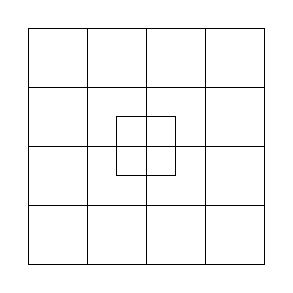
\begin{tikzpicture}[rotate=0,scale=0.75]
    \draw[] (0,0) rectangle (1,1);
    \draw[] (1,0) rectangle (2,1);
    \draw[] (2,0) rectangle (3,1);
    \draw[] (3,0) rectangle (4,1);
    
    \draw[] (0,1) rectangle (1,2);
    \draw[] (1,1) rectangle (2,2);
    \draw[] (2,1) rectangle (3,2);
    \draw[] (3,1) rectangle (4,2);
    
    \draw[] (0,2) rectangle (1,3);
    \draw[] (1,2) rectangle (2,3);
    \draw[] (2,2) rectangle (3,3);
    \draw[] (3,2) rectangle (4,3);
    
    \draw[] (0,3) rectangle (1,4);
    \draw[] (1,3) rectangle (2,4);
    \draw[] (2,3) rectangle (3,4);
    \draw[] (3,3) rectangle (4,4);
    
    \draw[] (1.5,1.5) rectangle (2.5,2.5);
    %\tkzDrawPolygon(O,A,B)
\end{tikzpicture}
\end{center}

\begin{multicols}{5}
\begin{enumerate}[label=\Alph* : ]
  \item $18 $
  \item $20 $
  \item $22 $
  \item $31 $
  \item $35 $
\end{enumerate}
\end{multicols}
\end{Exercise}
\begin{Answer}[ref=\ExerciseLabel]
E : 35\\\ws\\
Supposons que le carré a un côté de $4$ unités, il y a $4$ très petits carrés (de côté $0.5$), $17$ petits carrés (de côté $1$), $9$ moyens carrés (de côté $2$), $4$ grands carrés (de côté $3$) et $1$ très grand carré (de côté 4) ; $4+17+9+4+1=35$.
\end{Answer}

\begin{Exercise}[title={},label={\pktag\the\value{Exercise}}]
Si $p$ est un diviseur premier de $240$, alors forcément
\begin{multicols}{3}
\begin{enumerate}[label=\Alph* : ]
  \item $p $ divise 30;
  \item $p $ divise 48;
  \item $p $ divise 75;
  \item $p $ divise 80;
  \item Aucune des réponses
  \item[] précédentes.
\end{enumerate}
\end{multicols}
\end{Exercise}
\begin{Answer}[ref=\ExerciseLabel]
A : $p$ divise 30\\\ws\\
$240=2^4\cdot 3^1\cdot5^1$, donc $div_\text{premiers}240=\left\{2;3;5\right\}$, or les diviseurs premiers $2$, $3$ et $5$ divisent $30$.
\end{Answer}

\begin{Exercise}[title={\srp},label={\pktag\the\value{Exercise}}]
Dans figure imprécise suivante, l'angle $\widehat{AFD}$ mesure $94^\circ$ et les angles $\widehat{CIJ}$ et $\widehat{CJI}$ mesurent $80^\circ$. Que mesure, en degrés, $\widehat{FGH}+\widehat{GHI}$?

\begin{center}
\begin{tikzpicture}[rotate=14,scale=0.3]
    \tkzDefPoint(0,0){C}
    \tkzDefPoint(4,6){A}
    \tkzDefPoint(10,-2.5){B}
    \tkzDefPoint(9,4){D}
    \tkzDefPoint(4,-5){E}

    \tkzDrawSegments[](A,E A,B C,D E,D C,B)
    \tkzInterLL(C,D)(A,E)\tkzGetPoint{J}
    \tkzInterLL(A,B)(C,D)\tkzGetPoint{F}
    \tkzInterLL(D,E)(A,B)\tkzGetPoint{G}
    \tkzInterLL(D,E)(C,B)\tkzGetPoint{H}
    \tkzInterLL(C,B)(A,E)\tkzGetPoint{I}
    
    %\tkzLabelPoints(A,B,C,D,E,F,G,H,I,J)
    \tkzLabelPoints[left](A,C,J)
    \tkzLabelPoints[above](F)
    \tkzLabelPoints[below left](I)
    \tkzLabelPoints[below right](H)
    \tkzLabelPoints[right](G,D,B,E)
    %\tkzLabelSegments[below](O,B B,B2 B2,B3 B3,B4){1}
    %\tkzDrawPolygon(O,A,B)
\end{tikzpicture}
\end{center}

\end{Exercise}
\begin{Answer}[ref=\ExerciseLabel]
B : \\\ws\\
$FGHIJ$ est un pentagone $(n=5)$ et donc $\Sigma_\text{angles}=(n-2)\cdot180^\circ=(5-2)\cdot 180^\circ=3\cdot 180^\circ=540^\circ$.
\begin{align*}
&\widehat{FGH}+\widehat{GHI}+\widehat{HIJ}+\widehat{IJF}+\widehat{JFG}=540^\circ\\
\iff & \widehat{FGH}+\widehat{GHI} + \left(180^\circ-\widehat{CIJ}\right)+\left(180^\circ-\widehat{CJI}\right)+\widehat{AFD}=540^\circ\\
\iff & \widehat{FGH}+\widehat{GHI}+\left(180^\circ-80^\circ\right)+\left(180^\circ-80^\circ\right)+94^\circ=540^\circ\\
\iff&\widehat{FGH}+\widehat{GHI}+294^\circ=540^\circ\\
%\iff&\widehat{FGH}+\widehat{GHI}=540^\circ-294^\circ\\
\iff&\widehat{FGH}+\widehat{GHI}=246^\circ
\end{align*}

\end{Answer}

\begin{Exercise}[title={},label={\pktag\the\value{Exercise}}]
Audrey a aligné vingt pièces de $0.20\eur$ sur une table. Bernard a alors remplacé une pièce sur quatre, à partir de la 4\up{e}, par une pièce de $0.50\eur$. Ensuite, Charlotte a remplacé une pièce sur trois, à partir de la 3\up{e}, par une pièce de $1\eur$. Finalement, David a remplacé une pièce sur six, à partir de la 6\up{e}, par une pièce de $2\eur$. Quel est maintenant le montant total de la rangée de pièces de monnaie?
\begin{multicols}{3}
\begin{enumerate}[label=\Alph* : ]
  \item $10.5\eur $
  \item $12.2\eur $
  \item $13\eur $
  \item $13.5\eur $
  \item Une autre réponse.
  \item[]
\end{enumerate}
\end{multicols}
\end{Exercise}
\begin{Answer}[ref=\ExerciseLabel]
C : $13\eur$\\\ws
\begin{center}
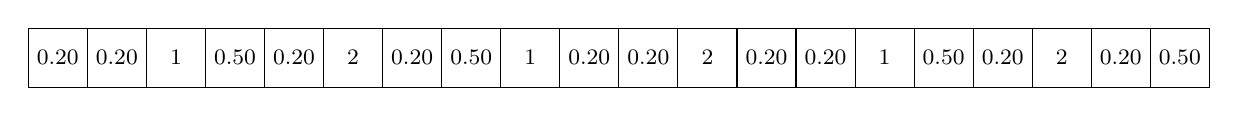
\begin{tikzpicture}[scale=0.75]
    \draw[] (0,0) rectangle (1,1) node[pos=.5] {\footnotesize{$0.20$}};
    \draw[] (1,0) rectangle (2,1) node[pos=.5] {\footnotesize{$0.20$}};
    \draw[] (2,0) rectangle (3,1) node[pos=.5] {\footnotesize{$1$}};
    \draw[] (3,0) rectangle (4,1) node[pos=.5] {\footnotesize{$0.50$}};
    \draw[] (4,0) rectangle (5,1) node[pos=.5] {\footnotesize{$0.20$}};
    \draw[] (5,0) rectangle (6,1) node[pos=.5] {\footnotesize{$2$}};
    \draw[] (6,0) rectangle (7,1) node[pos=.5] {\footnotesize{$0.20$}};
    \draw[] (7,0) rectangle (8,1) node[pos=.5] {\footnotesize{$0.50$}};
    \draw[] (8,0) rectangle (9,1) node[pos=.5] {\footnotesize{$1$}};
    \draw[] (9,0) rectangle (10,1) node[pos=.5] {\footnotesize{$0.20$}};
    \draw[] (10,0) rectangle (11,1) node[pos=.5] {\footnotesize{$0.20$}};
    \draw[] (11,0) rectangle (12,1) node[pos=.5] {\footnotesize{$2$}};
    \draw[] (12,0) rectangle (13,1) node[pos=.5] {\footnotesize{$0.20$}};
    \draw[] (13,0) rectangle (14,1) node[pos=.5] {\footnotesize{$0.20$}};
    \draw[] (14,0) rectangle (15,1) node[pos=.5] {\footnotesize{$1$}};
    \draw[] (15,0) rectangle (16,1) node[pos=.5] {\footnotesize{$0.50$}};
    \draw[] (16,0) rectangle (17,1) node[pos=.5] {\footnotesize{$0.20$}};
    \draw[] (17,0) rectangle (18,1) node[pos=.5] {\footnotesize{$2$}};
    \draw[] (18,0) rectangle (19,1) node[pos=.5] {\footnotesize{$0.20$}};
    \draw[] (19,0) rectangle (20,1) node[pos=.5] {\footnotesize{$0.50$}};
\end{tikzpicture}
\end{center}
$3\cdot2\eur+3\cdot1\eur+4\cdot0.5\eur+10\cdot0.2\eur=6\eur+3\eur+2\eur+2\eur=13\eur$
\end{Answer}

\begin{Exercise}[title={},label={\pktag\the\value{Exercise}}]
Le trapèze $ABCD$ vérifie: $(AB)\parallel (DC)$, $AB=AD$ et $DB=BC$. Si l'angle $\widehat{DAB}$ mesure $110^\circ$, que mesure l'angle $\widehat{ABC}$?
\begin{multicols}{3}
\begin{enumerate}[label=\Alph* : ]
  \item $135^\circ $
  \item $140^\circ $
  \item $145^\circ $
  \item $150^\circ $
  \item Une autre réponse.
  \item[]
\end{enumerate}
\end{multicols}
\end{Exercise}
\begin{Answer}[ref=\ExerciseLabel]
C : $135^\circ$\\\ws
\begin{center}
\begin{tikzpicture}[scale=1]
  \tkzDefPoint(0:0){D}
  \tkzDefPoint(70:3){A}
  \tkzDefPoint(35:5){B}
  \tkzDefPointBy[rotation=center B angle 110](D)\tkzGetPoint{C}
  
    \tkzMarkAngle[fill=myblue!40,size=0.55,opacity=1](D,A,B)
    \tkzMarkAngle[size=0.55,arc=l,opacity=1,arrows=,>=latex
    ](D,A,B)
    \tkzLabelAngle[pos=0.9](D,A,B){$110^\circ$}
    
    \tkzMarkAngle[fill=myblue!40,size=0.55,opacity=1](D,B,C)
    \tkzMarkAngle[size=0.55,arc=l,opacity=1,arrows=,>=latex
    ](D,B,C)
    \tkzLabelAngle[pos=0.8](D,B,C){$110^\circ$}
    
    \tkzMarkAngle[fill=myred!40,size=0.55,opacity=1](B,D,A)
    \tkzMarkAngle[size=0.55,arc=l,opacity=1,arrows=,>=latex
    ](B,D,A)
    \tkzLabelAngle[pos=1](B,D,A){$35^\circ$}
    
    \tkzMarkAngle[fill=myred!40,size=0.55,opacity=1](C,D,B)
    \tkzMarkAngle[size=0.55,arc=l,opacity=1,arrows=,>=latex
    ](C,D,B)
    \tkzLabelAngle[pos=1](C,D,B){$35^\circ$}
    
    \tkzMarkAngle[fill=myred!40,size=0.55,opacity=1](B,C,D)
    \tkzMarkAngle[size=0.55,arc=l,opacity=1,arrows=,>=latex
    ](B,C,D)
    \tkzLabelAngle[pos=1](B,C,D){$35^\circ$}
    
    \tkzMarkAngle[fill=myred!40,size=0.55,opacity=1](A,B,D)
    \tkzMarkAngle[size=0.55,arc=l,opacity=1,arrows=,>=latex
    ](A,B,D)
    \tkzLabelAngle[pos=1](A,B,D){$35^\circ$}
  \tkzDrawPolygon(A,B,C,D)
  \tkzDrawSegments(B,D)
  
  \tkzLabelPoint[above left](A){$A$}
  \tkzLabelPoint[above right](B){$B$}
  \tkzLabelPoint[below left](D){$D$}
  \tkzLabelPoint[below right](C){$C$}
  \tkzMarkSegments[mark=|](A,B A,D)
  \tkzMarkSegments[mark=||](B,D B,C)
  
\end{tikzpicture}
\end{center}
$\Delta ABD\sim\Delta BCD$, les triangles $ABD$ et $BCD$ sont semblables et donc $\widehat{DBC}=\widehat{DAB}=110^\circ$.\\
$\widehat{ABC}=\widehat{ABD}+\widehat{DBC}=\left(180^\circ-\widehat{DAB}\right):2+\widehat{DAB}=\left(180^\circ-110^\circ\right):2+110^\circ=35^\circ+110^\circ=145^\circ$
\end{Answer}

\begin{Exercise}[title={},label={\pktag\the\value{Exercise}}]
Dans la figure suivante, les points partagent les côtés sur lesquels ils se trouvent en segments de mêmes longueurs. L'aire du triangle $ABC$ est $180$; quelle est celle du triangle gris?

\begin{center}

\begin{tikzpicture}[scale=1]
    \tkzDefPoint(0:0){A}
    \tkzDefPoint(70:0.7){C1}
    \tkzDefPoint(70:1.4){C2}
    \tkzDefPoint(70:2.1){C3}
    \tkzDefPoint(70:2.8){C}
    
    \tkzDefPoint(0:1){B1}
    \tkzDefPoint(0:2){B2}
    \tkzDefPoint(0:3){B3}
    \tkzDefPoint(0:4){B4}
    \tkzDefPoint(0:5){B}
    
    \tkzDrawPolygon[fill=black!25](C2,B2,C3)
    \tkzDrawPolygon(A,B,C)
    
    \tkzLabelPoint[left](A){$A$}
    \tkzLabelPoint[above right](C){$C$}
    \tkzLabelPoint[right](B){$B$}
    
    \tkzDrawPoints[fill=black](A,B,C,C1,C2,C3,B1,B2,B3,B4)
  
\end{tikzpicture}
\end{center}

\begin{multicols}{5}
\begin{enumerate}[label=\Alph* : ]
  \item $9 $
  \item $18 $
  \item $27 $
  \item $36 $
  \item $45 $
\end{enumerate}
\end{multicols}
\end{Exercise}
\begin{Answer}[ref=\ExerciseLabel]
B : $18$\\\ws
\begin{center}
\begin{tikzpicture}[scale=1]
    \tkzDefPoint(0:0){A}
    \tkzDefPoint(70:0.7){C1}
    \tkzDefPoint(70:1.4){C2}
    \tkzDefPoint(70:2.1){C3}
    \tkzDefPoint(70:2.8){C}
    
    \tkzDefPoint(0:1){B1}
    \tkzDefPoint(0:2){B2}
    \tkzDefPoint(0:3){B3}
    \tkzDefPoint(0:4){B4}
    \tkzDefPoint(0:5){B}
    
    \tkzDefPointBy[projection=onto A--C](B2)\tkzGetPoint{H1}
    \tkzDefPointBy[projection=onto A--C](B)\tkzGetPoint{H2}
    
    \tkzDrawPolygon[fill=black!25](C2,B2,C3)
    \tkzDrawPolygon(A,B,C)
    
    \tkzDrawSegments[dashed](H1,B2 H2,B)
    \tkzLabelSegment[](H1,B2){$h$}
    \tkzLabelSegment[](H2,B){$H$}
    \tkzMarkRightAngle[draw=black,size=.15](B,H2,C);
    \tkzMarkRightAngle[draw=black,size=.15](B2,H1,C);

    \tkzLabelPoints[left](A)
    \tkzLabelPoint[above right](C){$C$}
    \tkzLabelPoint[right](B){$B$}
    
    \tkzDrawPoints[fill=black](A,B,C,C1,C2,C3,B1,B2,B3,B4)
\end{tikzpicture}
\end{center}
$A=\left(\frac{1}{4}\cdot AC\cdot h\right):2=\left(\frac{1}{4}\cdot AC\cdot \frac{2}{5}\cdot H\right):2=\frac{1}{10}\cdot AC\cdot H:2=\frac{1}{10}\cdot\frac{AC\cdot H}{2}=\frac{1}{10}\cdot[ABC]=\frac{1}{10}\cdot180=18$
\end{Answer}



\begin{Exercise}[title={},label={\pktag\the\value{Exercise}}]
La figure ci-dessous est un rectangle; que vaut $p+q$?
\begin{center}
\begin{tikzpicture}[scale=0.3]
\tkzInit[xmax=16,ymax=14,xmin=-1,ymin=-1]
    \tkzDrawXY[noticks]
    
    \tkzDefPoint(5,5){A}
    \tkzDefPoint(9,2){B}
    \tkzDefPoint(15,10){C}
    \tkzDefPoint(11,13){D}

    \tkzDrawPolygon(A,B,C,D)
    \tkzLabelPoint[left](A){$\left(5;5\right)$}
    \tkzLabelPoint[below](B){$\left(9;2\right)$}
    \tkzLabelPoint[right](C){$\left(15;q\right)$}
    \tkzLabelPoint[above](D){$\left(p;13\right)$}
    %\tkzClip
\end{tikzpicture}  
\end{center} 

\begin{multicols}{5}
\begin{enumerate}[label=\Alph* : ]
  \item $17 $
  \item $18 $
  \item $20 $
  \item $21 $
  \item $22 $
\end{enumerate}
\end{multicols}

\end{Exercise}
\begin{Answer}[ref=\ExerciseLabel]
D : $21$\\\ws
\begin{center}
\begin{tikzpicture}[scale=0.3]
\tkzInit[xmax=16,ymax=14,xmin=-1,ymin=-1]
    \tkzDrawXY[noticks]
    
    \tkzDefPoint(5,5){A}
    \tkzDefPoint(9,2){B}
    \tkzDefPoint(15,10){C}
    \tkzDefPoint(11,13){D}

    \tkzDrawPolygon(A,B,C,D)
    \tkzLabelPoint[left](A){$\left(5;5\right)$}
    \tkzLabelPoint[below](B){$\left(9;2\right)$}
    \tkzLabelPoint[right](C){$\left(15;\textbf{10}\right)$}
    \tkzLabelPoint[above](D){$\left(\textbf{11};13\right)$}
    %\tkzClip
\end{tikzpicture}  
\end{center} 
$p=11$ et $q=10$ ; ainsi $p+q=11+10=21$.
\end{Answer}

% %%%%%%%%%%%%%%%%%%%%%%%%%%%%%%%%%%%%%%%%%%%%%%%%%%%%%%%%%%%%%%%%
% %====================================================================
\ifstandalone
    \chapitre{Solutions}\shipoutAnswer%\finchapitre
\else
% 
\fi
% %====================================================================
\end{document}